%%Modelo de TCC da UFVJM
%%Este modelo segue a Resolução no. 15 do CONSEPE, de 21 de Maio de 2010. 
%%LEIA a Resolução!
%%Vide: http://www.ufvjm.edu.br/prograd/tcc.html
%%----
%%Configuração Padrão
%%a4paper - (Tamanho do papel: A4)
%%12pt - (Tamanho da fonte: 12pt)
%%twoside - (Impressão frente e verso)
%%openright - Todos os capítulos começam no anverso da folha (coincide com as páginas ímpares).
%%            Para essa opção funcionar como esperado, você DEVE USAR JUNTO com a opção twoside.
%%            Se necessário, coloca uma página par em branco para forçar o 
%%            começo do próximo capítulo em uma página ímpar.
%%capitulomaiusculo - Fixa em maiúsculo o título de todos os capítulos com numeração (comando \chapter). 
%%                    O título dos capítulos sem numeração (comando \chapter*) fica em maiúsculo,
%%                    independente dessa opção.
%%Obs.: Esse modelo usa o arquivo "tcc-ufvjm.cls". Por praticidade, deixe esse arquivo 
%%      na mesma pasta que o arquivo principal do seu trabalho.
\documentclass[a4paper,12pt,twoside,openright,capitulomaiusculo]{tcc-ufvjm}

%%Fonte Times New Roman.
\usepackage{mathptmx}

\usepackage{amsmath,amsthm,amsfonts,amssymb}
\usepackage{graphicx}
\usepackage[mathcal]{eucal}
\usepackage{latexsym}
\usepackage[brazil]{babel}

%%USE A CODIFICAÇÃO UTF-8 na formatação dos seus arquivos.
%%MUDE a opção "utf8" caso altere a codificação.
\usepackage[utf8]{inputenc}

\usepackage{bm}
\usepackage[all]{xy}

%%Pacote para Gerar o Índice.
%%Obs.: * O Índice é opcional. Se não quiser utilizar, basta colocar % na frente da linha.
%%      * Além disso, coloque % na frente da linha que contém \printindex (que está próximo ao fim desse arquivo).
\usepackage{makeidx}\makeindex

%%Pacote para gerar a referência no padrão ABNT
%%Página do projeto: http://code.google.com/p/abntex2/
%%Obs.: * Esse pacote usa os arquivos: abntex2cite.sty, abntex2abrev.sty, abntex2-options.bib,
%%      abntex2-alf.bst e abntex2-num.bst.
%%      * Esses arquivos estão na pasta pos-textual/referencias. NÃO TROQUE de pasta esses arquivos, 
%%      pois caso contrário será necessário editá-los.
\usepackage[alf]{pos-textual/referencias/abntex2cite}

%-----------------------------------------------------------
%-----------------------------------------------------------
\theoremstyle{plain}
\newtheorem{theorem}{Teorema}[section]
\newtheorem{axiom}{Axioma}[section]
\newtheorem{corollary}{Corolário}[section]
\newtheorem{lemma}{Lema}[section]
\newtheorem{proposition}{Proposição}[section]
%-----------------------------------------------------------
\theoremstyle{definition}
\newtheorem{definition}{Definição}[section]
\newtheorem{example}{Exemplo}[section]
%-----------------------------------------------------------
\theoremstyle{remark}
\newtheorem{remark}{Observação}[section]
%-----------------------------------------------------------
%-----------------------------------------------------------
\newcommand{\R}{\mathbb{R}}
\newcommand{\N}{\mathbb{N}}
\newcommand{\Z}{\mathbb{Z}}
\newcommand{\Q}{\mathbb{Q}}
\newcommand{\K}{\mathbb{K}}
\newcommand{\I}{\mathbb{I}}
\newcommand{\id}{\mathbf{1}}
\newcommand{\U}{\mathcal{U}}
\newcommand{\V}{{\cal V}}
%-----------------------------------------------------------
\def\ind{\hbox{ ind }}
%-----------------------------------------------------------
\begin{document}

%%---- ELEMENTOS PRÉ-TEXTUAIS ----

%%(Opcional) Inserir uma imagem de fundo na capa do trabalho.
%% Obs.: retire o caracter % no início da linha abaixo caso queira inserir uma imagem.
%\fundodacapa{figuras/minha-imagem.png}

%%Informações sobre a Instituição.
\instituicao{Universidade Federal dos Vales do Jequitinhonha e Mucuri}
\sigla{UFVJM}
\instituicaoendereco{Campus do Mucuri - Rua do Cruzeiro, n. 01 - Jardim São Paulo - CEP 39803-371.}
\unidadeacademica{Faculdade de Ciências Sociais Aplicadas e Exatas}

%%Informação sobre o Curso.
\curso{Licenciatura em Matemática}

%%Local e Ano.
\cidade{Teófilo Otoni}
\ano{2014}

%%Título e subtítulo (caso exista).
\titulo{O título ficará maiúsculo e em negrito:}
%Subtitulo (Opcional) - Coloque um % na frente da linha abaixo caso não haja subtítulo.
\subtitulo{e o subtítulo (quando houver) ficará minúsculo, sendo separado do título por dois pontos.}

%%Autor(es)
%%Obs.: * Para reduzir o número de autores, basta colocar % na frente das linhas correspondentes.
%%      * Esse modelo suporta no máximo 6 autores. Se seu curso permitir mais, 
%%        será necessário editar o arquivo "tcc-ufvjm.cls".
\nomeautorum{Nome do}\sobrenomeautorum{Autor}
\emailautorum{e-mail@dominio.com.br}

% \nomeautordois{Nome do}\sobrenomeautordois{Autor 2}
% \emailautordois{e-mail2@dominio.com.br}
% 
% \nomeautortres{Nome do}\sobrenomeautortres{Autor 3}
% \emailautortres{e-mail3@dominio.com.br}
% 
% \nomeautorquatro{Nome do}\sobrenomeautorquatro{Autor 4}
% \emailautorquatro{e-mail4@dominio.com.br}
% 
% \nomeautorcinco{Nome do}\sobrenomeautorcinco{Autor 5}
% \emailautorcinco{e-mail5@dominio.com.br}
% 
% \nomeautorseis{Nome do}\sobrenomeautorseis{Autor 6}
% \emailautorseis{e-mail6@dominio.com.br}

%%Nome do Orientador, 1o. Avaliador e 2o. Avaliador. 
%%Obs.: * Co-orientador, 3o., 4o. e 5o. Avaliadores são opcionais. Caso não tenha, basta colocar % na frente das linhas correspondentes.
%%      * Esse modelo suporta no máximo 6 avaliadores (o orientador e mais cinco). Se seu TCC tiver mais, 
%%        será necessário editar o arquivo "tcc-ufvjm.cls".
\orientador{Nome do Orientador(a)}
\ttorientador{Prof. Dr.}
\instorientador{Instituição}

% \coorientador{Nome do Co-orientador(a)}
% \ttcoorientador{Prof. Dr.}
% \instcoorientador{Instituição}

\examinadorum{Nome do Avaliador(a) 1}
\ttexaminadorum{Prof. Dr.}
\instexaminadorum{Instituição}

\examinadordois{Nome do Avaliador(a) 2}
\ttexaminadordois{Prof. Dr.}
\instexaminadordois{Instituição}

% \examinadortres{Nome do Avaliador(a) 3}
% \ttexaminadortres{Prof. Dr.}
% \instexaminadortres{Instituição}
% 
% \examinadorquatro{Nome do Avaliador(a) 4}
% \ttexaminadorquatro{Prof. Dr.}
% \instexaminadorquatro{Instituição}
% 
% \examinadorcinco{Nome do Avaliador(a) 5}
% \ttexaminadorcinco{Prof. Dr.}
% \instexaminadorcinco{Instituição}

%%O número CDU será obtido na Biblioteca, depois da versão final do TCC.
%%Caso não queira gerar a ficha catalográfica, basta colocar % na frente das próximas linhas.
%%Se a ficha catalográfica não for gerada, no seu lugar haverá uma página em branco (contendo apenas a numeração ii)
\CDU{xxx.xx} %substitua xxx.xx pelo número informado pela Biblioteca.
\areas{1. Primeira Área 1; 2. Segunda Área; Terceira Área; Quarta Área 4.} %coloque a(s) área(s) de seu trabalho.
\npaginas{xx} %substitua xx pelo total de páginas do trabalho 
%%             Não contabilizar os elementos pré-textuais: capa, folha de rosto, agradecimento, 
%%             epígrafe, resumo, etc.

%%Errata (Opcional)
%%Obs.: * A Errata deve aparecer ANTES do comando \maketitle
%%      * Se não houver Errata, apenas coloque % na frente da próxima linha.
\errata{

SOBRENOME, Nome. \textbf{Título da obra 1}. Editora. Cidade, Ano.

\begin{center}
\begin{tabular}{llll}
 Página & Linha & Onde se lê: & Leia-se:\\
 10     & 10    & tete        & teste \\
 27     & 12    & tete        & teste \\
 11     & 05    & tete        & teste
\end{tabular}
\end{center}

SOBRENOME, Nome. \textbf{Título da obra 2}. Editora. Cidade, Ano.

\begin{center}
\begin{tabular}{llll}
 Página & Linha & Onde se lê: & Leia-se:\\
 10     & 10    & tete        & teste \\
 27     & 12    & tete        & teste \\
 11     & 05    & tete        & teste
\end{tabular}
\end{center}

SOBRENOME, Nome. \textbf{Título da obra 3}. Editora. Cidade, Ano.

\begin{center}
\begin{tabular}{llll}
 Página & Linha & Onde se lê: & Leia-se:\\
 10     & 10    & tete        & teste \\
 27     & 12    & tete        & teste \\
 11     & 05    & tete        & teste
\end{tabular}
\end{center}

SOBRENOME, Nome. \textbf{Título da obra n}. Editora. Cidade, Ano.

\begin{center}
\begin{tabular}{llll}
 Página & Linha & Onde se lê: & Leia-se:\\
 10     & 10    & tete        & teste \\
 27     & 12    & tete        & teste \\
 11     & 05    & tete        & teste
\end{tabular}
\end{center}
}

%%Gerar: Capa, Folha de Rosto, Errata (caso \errata seja definido), 
%%       Ficha Catalográfica (caso \CDU seja definido) e Folha de Aprovação.
\maketitle

\begin{dedicatoria}
À Francislene e Ana, por toda alegria que há em mim.
\end{dedicatoria} %opcional
\begin{agradecimento}
Aos colegas, pela diversão e (às vezes) estudo.

Ao professor Nome do Orientador(a) pela orientação, amizade e
principalmente pela paciência, sem a qual este trabalho não se
realizaria.

Aos professores e funcionários do Nome do Departamento, que durante esses anos 
contribuíram de algum modo para o nosso enriquecimento pessoal e
profissional.
\end{agradecimento} %opcional
\begin{epigrafe}
``Sem esforço, não há ganho''.

\hfill Dito Popular.
\end{epigrafe} %opcional
\begin{resumo}
Seu resumo em português.

\noindent \textbf{Palavras-chave:} Palavra 1, Palavra 2, Palavra 3, Palavra 4.
\end{resumo} %obrigatório
\begin{resumo}[Abstract]
Seu resumo em inglês.

\noindent \textbf{Keywords:} Palavra 1, Palavra 2, Palavra 3, Palavra 4.
\end{resumo} %obrigatório
\listadefiguras %opcional
\listadetabelas %opcional
\begin{abreviaturas}
%Use uma linha em branco para separar cada uma das abreviaturas.
%Obs.: Dentro do ambiente "abreviaturas" o início dos parágrafos não fica recuado.

    Dr. - Doutor.

    Me. - Mestre.

    MSc. - Master of Science.

    PhD. - Doctor of Philosophy. 

\end{abreviaturas} %opcional
\begin{siglas}
%Use uma linha em branco para separar cada uma das siglas.
%Obs.: Dentro do ambiente "siglas" o início dos parágrafos não fica recuado.

    MEC - Ministério da Educação.

    UFVJM - Universidade Federal dos Vales do Jequitinhonha e Mucuri.

\end{siglas} %opcional
\begin{simbolos}
%Use uma linha em branco para separar cada um dos símbolos.

    $\neq$ - Diferente.

    $\notin$ - Não pertence.

\end{simbolos} %opcional
\sumario %obrigatório

%%---- ELEMENTOS TEXTUAIS ----

\chapter{Introdução.}

Aqui vai a introdução do trabalho\ldots 

(Estava óbvio, não estava? ;))
\chapter{Revisão de Literatura (ou Referencial Teórico).}

O que já tem escrito no tema que você escolheu?

\section{Primeira seção da Revisão}

Para incluir uma referência em seu trabalho, como por exemplo \cite{Autor1}, use o comando \verb!\cite{<rótulo>}!, 
onde \verb!<rótulo>! indica uma referência que você criou no arquivo \verb!referencias.bib! (que está na pasta \verb!pos-textual/referencias!). 
Um outro exemplo de referência com mais de três autores \cite{Autor3}.

Se você quiser fazer uma citação com mais de três linhas, use o ambiente \verb!citacao!. Veja um exemplo abaixo.

\begin{citacao}
A citação com mais de três linhas tem fonte com tamanho 10 pt, espaço simples entre 
linhas e recuo de 4 cm da margem esquerda. A citação com mais de três linhas tem fonte 
com tamanho 10 pt, espaço simples entre linhas e recuo de 4 cm da margem esquerda. 
A citação com mais de três linhas tem fonte com tamanho 10 pt, espaço simples entre 
linhas e recuo de 4 cm da margem esquerda. A citação com mais de três linhas tem fonte 
com tamanho 10 pt, espaço simples entre linhas e recuo de 4 cm da margem esquerda \cite[p. 11]{Autor2}. 
(Observação: para indicar a página na referência, como ``p. 11'' nesse exemplo, use o 
comando \verb!\cite[p. 11]{<rótulo>}!.)
\end{citacao}

A Tabela~\ref{tabelateste1} é um exemplo de como ficará uma tabela no seu texto. Note que a 
legenda fica na parte superior e tem fonte com tamanho 10 pt (além de espaço simples entre linhas, como 
você pode notar na Tabela~\ref{tabelateste2}).

\begin{table}[htb]
 \centering
 \caption{Exemplo de tabela.}
 \begin{tabular}{|c|c|c|c|}
  \hline
  Teste 1 & Teste 2 & Teste 3 & Teste 4\\ \hline
  Teste 1 & Teste 2 & Teste 3 & Teste 4\\ \hline
  Teste 1 & Teste 2 & Teste 3 & Teste 4\\ \hline
  Teste 1 & Teste 2 & Teste 3 & Teste 4\\ \hline
 \end{tabular}
 \label{tabelateste1}
\end{table}

\begin{table}[htb]
 \centering
 \caption[Legenda mais curta.]{Esse é um exemplo de tabela com legenda muito grande, que tem por objetivo mostrar como o espaço entre linhas será simples.}
 \begin{tabular}{|c|c|c|c|}
  \hline
  Teste 1 & Teste 2 & Teste 3 & Teste 4\\ \hline
  Teste 1 & Teste 2 & Teste 3 & Teste 4\\ \hline
  Teste 1 & Teste 2 & Teste 3 & Teste 4\\ \hline
  Teste 1 & Teste 2 & Teste 3 & Teste 4\\ \hline
 \end{tabular}
 \label{tabelateste2}
\end{table}

\subsection{Exemplo de Subseção.}

Esse é um exemplo de subseção.

E aqui temos um exemplo de nota de rodapé \footnote{As notas no rodapé 
tem fonte com tamanho 10 pt e espaço simples entre linhas. O filete (linha) que separa as notas do resto 
do texto tem tamanho de 3 cm.}.

A Figura~\ref{figurateste1} é um exemplo de como ficará uma figura no seu texto\index{exemplo de figura}. Note que a 
legenda fica na parte inferior e tem fonte com tamanho 10 pt (além de espaço simples entre linhas, como 
você pode notar na Figura~\ref{figurateste2})
%Note que o comando \index é usado para inserir "exemplo de figura" no Índice.


\begin{figure}[htb]
 \centering
 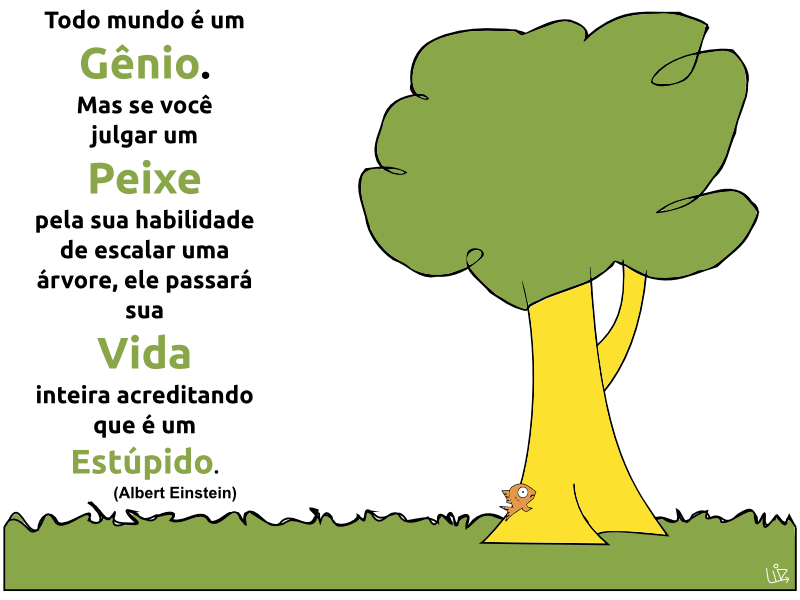
\includegraphics[scale=0.4]{figuras/todos-somos-genios}
 \caption{Exemplo de Figura.}
 \label{figurateste1}
\end{figure}

\begin{figure}[htb]
 \centering
  
\includegraphics[scale=0.8]{figuras/tux}
  \caption[Legenda mais curta.]{Esse é um exemplo de figura com legenda muito grande, que tem por objetivo mostrar como o espaço entre linhas será simples.}
  \label{figurateste2}
\end{figure}

\section{Segunda seção da Revisão.}

Em \eqref{equacao1} temos um exemplo de texto matemático com numeração\index{equação com numeração}. E logo depois 
temos um exemplo de texto matemático sem numeração.
%Note que o comando \index é usado para inserir "equação com numeração" no Índice.

\begin{equation}\label{equacao1}
 \int_a^b f'(x)\,dx = f(b) - f(a)
\end{equation}

\begin{equation}\nonumber
 \int_a^b f'(x)\,dx = f(b) - f(a)
\end{equation}

Aqui está mais outro exemplo de referência \cite{Autor4}.
\chapter{Material e Métodos (ou Metodologia).}

Como você realizou seu trabalho?

\section{Primeira seção da Metodologia}

Texto da primeira seção.

\section{Segunda seção da Metodologia.}

Texto da segunda seção.
\chapter{Resultados.}

Quais foram os resultados que você obteve com o seu trabalho?

\section{Primeira seção dos Resultados.}

Texto da primeira seção.

\section{Segunda seção dos Resultados.}

Texto da segunda seção.

\chapter{Discussão.}

Discuta aqui os resultados do seu trabalho\index{equação com numeração!outro teste}.
%Note que o comando \index é usado para inserir "outro teste" como subitem de "equação com numeração" no Índice.

\section{Primeira seção da Discussão.}

Texto da primeira seção.

\section{Segunda seção da Discussão.}

Texto da segunda seção.

\chapter{Conclusão.}

Aponte aqui as conclusões do seu trabalho.

\chapter{Considerações Finais (Opcional).}

Citar aqui trabalhos futuros e outras considerações.



%%---- ELEMENTOS PÓS-TEXTUAIS ----

%%Referências
%%Para adicionar referências, você precisa editar o arquivo "referencias.bib" na pasta "pos-textual/referencias".
\bibliography{pos-textual/referencias/referencias}

%%O Glossário é opcional. Caso não tenha, basta colocar % na frente da próxima linha.
\begin{glossario}
%Use uma linha em branco para separar cada um dos itens no glossário.

\textbf{PALAVRA 1} - Defina o significado da palavra 1.

\textbf{PALAVRA 2} - Defina o significado da palavra 2.

\end{glossario}

%%O Apêndice é opcional. Caso não tenha, basta colocar % na frente da próxima linha.
%%Obs.: antes de incluir o Apêndice, você PRECISA colocar o comando \iniciarapendice. 
\iniciarapendice
\chapter{Primeiro Apêndice}

Texto do primeiro apêndice.

\chapter{Segundo Apêndice}

Texto do segundo apêndice.

%%O Anexo é opcional. Caso não tenha, basta colocar % na frente da próxima linha.
%%Obs.: antes de incluir o Anexo, você PRECISA colocar o comando \iniciaranexo.
\iniciaranexo
\chapter{Primeiro Anexo}

Texto do primeiro anexo.

\chapter{Segundo Anexo}

Texto do segundo anexo.

%%O Índice é opcional. 
%%Obs.: Caso não tenha, basta colocar % na frente da próxima linha.
\printindex

%%A Autorização para Reprodução é obrigatória.
\exibirautorizacao

%%(Opcional) %Inserir uma última página com um fundo personalizado.
%\inserirpaginacomfundo{figuras/minha-imagem.png}
\end{document}